
\documentclass[letterpaper,hide notes,xcolor={table,svgnames},pdftex,10pt]{beamer}
\def\showexamples{t}


%\usepackage[svgnames]{xcolor}

%% Demo talk
%\documentclass[letterpaper,notes=show]{beamer}

\usecolortheme{crane}
\setbeamertemplate{navigation symbols}{}

\usetheme{MyPittsburgh}
%\usetheme{Frankfurt}

%\usepackage{tipa}

\usepackage{hyperref}
\usepackage{graphicx,xspace}
\usepackage[normalem]{ulem}
\usepackage{multicol}
\usepackage{amsmath,amssymb,amsthm,graphicx,xspace}
\newcommand\SF[1]{$\bigstar$\footnote{SF: #1}}

\usepackage[default]{sourcesanspro}
\usepackage[T1]{fontenc}
\usepackage[scaled]{beramono}
\usepackage{tikzpagenodes}

\newcounter{tmpnumSlide}
\newcounter{tmpnumNote}


% old question code
%\newcommand\question[1]{{$\bigstar$ \small \onlySlide{2}{#1}}}
% \newcommand\nquestion[1]{\ifdefined \presentationonly \textcircled{?} \fi \note{\par{\Large \textbf{?}} #1}}
% \newcommand\nanswer[1]{\note{\par{\Large \textbf{A}} #1}}


 \newcommand\mnote[1]{%
   \addtocounter{tmpnumSlide}{1}
   \ifdefined\showcues {~\tiny\fbox{\arabic{tmpnumSlide}}}\fi
   \note{\setlength{\parskip}{1ex}\addtocounter{tmpnumNote}{1}\textbf{\Large \arabic{tmpnumNote}:} {#1\par}}}

\newcommand\mmnote[1]{\note{\setlength{\parskip}{1ex}#1\par}}

%\newcommand\mnote[2][]{\ifdefined\handoutwithnotes {~\tiny\fbox{#1}}\fi
% \note{\setlength{\parskip}{1ex}\textbf{\Large #1:} #2\par}}

%\newcommand\mnote[2][]{{\tiny\fbox{#1}} \note{\setlength{\parskip}{1ex}\textbf{\Large #1:} #2\par}}

\newcommand\mquestion[2]{{~\color{red}\fbox{?}}\note{\setlength{\parskip}{1ex}\par{\Large \textbf{?}} #1} \note{\setlength{\parskip}{1ex}\par{\Large \textbf{A}} #2\par}\ifdefined \presentationonly \pause \fi}

\newcommand\blackboard[1]{%
\ifdefined   \showblackboard
  {#1}
  \else {\begin{center} \fbox{\colorbox{blue!30}{%
         \begin{minipage}{.95\linewidth}%
           \hspace{\stretch{1}} Some space intentionally left blank; done at the blackboard.%
         \end{minipage}}}\end{center}}%
         \fi%
}



%\newcommand\q{\tikz \node[thick,color=black,shape=circle]{?};}
%\newcommand\q{\ifdefined \presentationonly \textcircled{?} \fi}

\usepackage{listings}
\lstset{basicstyle=\footnotesize\ttfamily,
	breaklines=true,
	aboveskip=15pt,
  	belowskip=15pt,
	frame=lines,
	numbers=left, basicstyle=\scriptsize, numberstyle=\tiny, stepnumber=0, numbersep=2pt
}

\usepackage{siunitx}
\newcommand\sius[1]{\num[group-separator = {,}]{#1}\si{\micro\second}}
\newcommand\sims[1]{\num[group-separator = {,}]{#1}\si{\milli\second}}
\newcommand\sins[1]{\num[group-separator = {,}]{#1}\si{\nano\second}}
\sisetup{group-separator = {,}, group-digits = true}

%% -------------------- tikz --------------------
\usepackage{tikz}
\usetikzlibrary{positioning}
\usetikzlibrary{arrows,backgrounds,automata,decorations.shapes,decorations.pathmorphing,decorations.markings,decorations.text,decorations.pathreplacing}

\tikzstyle{place}=[circle,draw=blue!50,fill=blue!20,thick, inner sep=0pt,minimum size=6mm]
\tikzstyle{transition}=[rectangle,draw=black!50,fill=black!20,thick, inner sep=0pt,minimum size=4mm]

\tikzstyle{block}=[rectangle,draw=black, thick, inner sep=5pt]
\tikzstyle{bullet}=[circle,draw=black, fill=black, thin, inner sep=2pt]

\tikzstyle{pre}=[<-,shorten <=1pt,>=stealth',semithick]
\tikzstyle{post}=[->,shorten >=1pt,>=stealth',semithick]
\tikzstyle{bi}=[<->,shorten >=1pt,shorten <=1pt, >=stealth',semithick]

\tikzstyle{mut}=[-,>=stealth',semithick]

\tikzstyle{treereset}=[dashed,->, shorten >=1pt,>=stealth',thin]

\usepackage{ifmtarg}
\usepackage{xifthen}
\makeatletter
% new counter to now which frame it is within the sequence
\newcounter{multiframecounter}
% initialize buffer for previously used frame title
\gdef\lastframetitle{\textit{undefined}}
% new environment for a multi-frame
\newenvironment{multiframe}[1][]{%
\ifthenelse{\isempty{#1}}{%
% if no frame title was set via optional parameter,
% only increase sequence counter by 1
\addtocounter{multiframecounter}{1}%
}{%
% new frame title has been provided, thus
% reset sequence counter to 1 and buffer frame title for later use
\setcounter{multiframecounter}{1}%
\gdef\lastframetitle{#1}%
}%
% start conventional frame environment and
% automatically set frame title followed by sequence counter
\begin{frame}%
\frametitle{\lastframetitle~{\normalfont(\arabic{multiframecounter})}}%
}{%
\end{frame}%
}
\makeatother

\makeatletter
\newdimen\tu@tmpa%
\newdimen\ydiffl%
\newdimen\xdiffl%
\newcommand\ydiff[2]{%
    \coordinate (tmpnamea) at (#1);%
    \coordinate (tmpnameb) at (#2);%
    \pgfextracty{\tu@tmpa}{\pgfpointanchor{tmpnamea}{center}}%
    \pgfextracty{\ydiffl}{\pgfpointanchor{tmpnameb}{center}}%
    \advance\ydiffl by -\tu@tmpa%
}
\newcommand\xdiff[2]{%
    \coordinate (tmpnamea) at (#1);%
    \coordinate (tmpnameb) at (#2);%
    \pgfextractx{\tu@tmpa}{\pgfpointanchor{tmpnamea}{center}}%
    \pgfextractx{\xdiffl}{\pgfpointanchor{tmpnameb}{center}}%
    \advance\xdiffl by -\tu@tmpa%
}
\makeatother
\newcommand{\copyrightbox}[3][r]{%
\begin{tikzpicture}%
\node[inner sep=0pt,minimum size=2em](ciimage){#2};
\usefont{OT1}{phv}{n}{n}\fontsize{4}{4}\selectfont
\ydiff{ciimage.south}{ciimage.north}
\xdiff{ciimage.west}{ciimage.east}
\ifthenelse{\equal{#1}{r}}{%
\node[inner sep=0pt,right=1ex of ciimage.south east,anchor=north west,rotate=90]%
{\raggedleft\color{black!50}\parbox{\the\ydiffl}{\raggedright{}#3}};%
}{%
\ifthenelse{\equal{#1}{l}}{%
\node[inner sep=0pt,right=1ex of ciimage.south west,anchor=south west,rotate=90]%
{\raggedleft\color{black!50}\parbox{\the\ydiffl}{\raggedright{}#3}};%
}{%
\node[inner sep=0pt,below=1ex of ciimage.south west,anchor=north west]%
{\raggedleft\color{black!50}\parbox{\the\xdiffl}{\raggedright{}#3}};%
}
}
\end{tikzpicture}
}


%% --------------------

%\usepackage[excludeor]{everyhook}
%\PushPreHook{par}{\setbox0=\lastbox\llap{MUH}}\box0}

%\vspace*{\stretch{1}

%\setbox0=\lastbox \llap{\textbullet\enskip}\box0}

\setlength{\parskip}{\fill}

\newcommand\noskips{\setlength{\parskip}{1ex}}
\newcommand\doskips{\setlength{\parskip}{\fill}}

\newcommand\xx{\par\vspace*{\stretch{1}}\par}
\newcommand\xxs{\par\vspace*{2ex}\par}
\newcommand\tuple[1]{\langle #1 \rangle}
\newcommand\code[1]{{\sf \footnotesize #1}}
\newcommand\ex[1]{\uline{Example:} \ifdefined \presentationonly \pause \fi
  \ifdefined\showexamples#1\xspace\else{\uline{\hspace*{2cm}}}\fi}

\newcommand\ceil[1]{\lceil #1 \rceil}


\AtBeginSection[]
{
   \begin{frame}
       \frametitle{Outline}
       \tableofcontents[currentsection]
   \end{frame}
}



\pgfdeclarelayer{edgelayer}
\pgfdeclarelayer{nodelayer}
\pgfsetlayers{edgelayer,nodelayer,main}

\tikzstyle{none}=[inner sep=0pt]
\tikzstyle{rn}=[circle,fill=Red,draw=Black,line width=0.8 pt]
\tikzstyle{gn}=[circle,fill=Lime,draw=Black,line width=0.8 pt]
\tikzstyle{yn}=[circle,fill=Yellow,draw=Black,line width=0.8 pt]
\tikzstyle{empty}=[circle,fill=White,draw=Black]
\tikzstyle{bw} = [rectangle, draw, fill=blue!20, 
    text width=4em, text centered, rounded corners, minimum height=2em]
    
    \newcommand{\CcNote}[1]{% longname
	This work is licensed under the \textit{Creative Commons #1 3.0 License}.%
}
\newcommand{\CcImageBy}[1]{%
	\includegraphics[scale=#1]{creative_commons/cc_by_30.pdf}%
}
\newcommand{\CcImageSa}[1]{%
	\includegraphics[scale=#1]{creative_commons/cc_sa_30.pdf}%
}
\newcommand{\CcImageNc}[1]{%
	\includegraphics[scale=#1]{creative_commons/cc_nc_30.pdf}%
}
\newcommand{\CcGroupBySa}[2]{% zoom, gap
	\CcImageBy{#1}\hspace*{#2}\CcImageNc{#1}\hspace*{#2}\CcImageSa{#1}%
}
\newcommand{\CcLongnameByNcSa}{Attribution-NonCommercial-ShareAlike}

\newenvironment{changemargin}[1]{% 
  \begin{list}{}{% 
    \setlength{\topsep}{0pt}% 
    \setlength{\leftmargin}{#1}% 
    \setlength{\rightmargin}{1em}
    \setlength{\listparindent}{\parindent}% 
    \setlength{\itemindent}{\parindent}% 
    \setlength{\parsep}{\parskip}% 
  }% 
  \item[]}{\end{list}} 




\title{Lecture 25 --- Profiling }

\author{Patrick Lam \\ \small \texttt{patrick.lam@uwaterloo.ca}}
\institute{Department of Electrical and Computer Engineering \\
  University of Waterloo}
\date{\today}


\begin{document}

\begin{frame}
  \titlepage

 \end{frame}


\begin{frame}
\frametitle{Remember the Initial Quiz}


Think back: what operations are fast and what operations are not?

Takeaway: our intuition  is often wrong. 

Not just at a macro level, \\
but at a micro level. 

You may be able to narrow down that this computation of $x$ is slow, \\
but if you examine it carefully\ldots what parts of it are slow?


\end{frame}



\begin{frame}
\frametitle{Premature Optimization}

\vspace*{.5cm}

\begin{quote}
\textit{Programmers waste enormous amounts of time thinking about, or worrying about, the speed of noncritical parts of their programs, and these attempts at efficiency actually have a strong negative impact when debugging and maintenance are considered. We should forget about small efficiencies, say about 97\% of the time: premature optimization is the root of all evil. Yet we should not pass up our opportunities in that critical 3\%.}
\end{quote}
	\hfill -- Donald Knuth


\end{frame}



\begin{frame}
\frametitle{That Saying You Were Expecting}


\begin{changemargin}{1.5cm}
Feeling lucky? \\
Maybe you optimized a slow part. 

\begin{center}
	
\includegraphics[width=0.4\textwidth]{images/feellucky.jpg}
\end{center}

To make your programs or systems fast, \\
you need to find out what is currently slow and improve it (duh!). 

Up until now, it's mostly been about \\
\qquad ``let's speed this up''.\\
We haven't taken much time to decide what we should speed up.
\end{changemargin}

\end{frame}



\begin{frame}
\frametitle{Basic Overview}


\begin{changemargin}{1.5cm}
General idea:\\
\qquad collect data on what parts of the code\\
\qquad are taking up most of the time.

\begin{itemize}
\item What functions get called?
\item How long do functions take?
\item What's using memory?
\end{itemize}
\end{changemargin}

\end{frame}



\begin{frame}
\frametitle{\texttt{printf}}


\begin{changemargin}{1.5cm}
There is always the ``informal'' way: ``debug'' by print statements.

On entry to \texttt{foo}, log ``entering function foo'', plus timestamp.

On exit, log ``exiting foo'', also with timestamp.
\end{changemargin}

\begin{center}
	
\includegraphics[width=0.5\textwidth]{images/stringerbell.jpg}
\end{center}

\end{frame}



\begin{frame}
\frametitle{Console Profiling}


\begin{changemargin}{1cm}
Kind of works, and [JZ] has used it... But this approach is not necessarily good.  

This is ``invasive'' profiling---change the source code of the program to add instrumentation (log statements). 

Plus we have to do a lot of manual accounting.

Doesn't really scale.
\end{changemargin}

\end{frame}



\begin{frame}
\frametitle{Wizardry!}


\begin{changemargin}{2cm}
Like debugging: if you get to be a wizard you can maybe do it by code inspection.

\begin{center}
	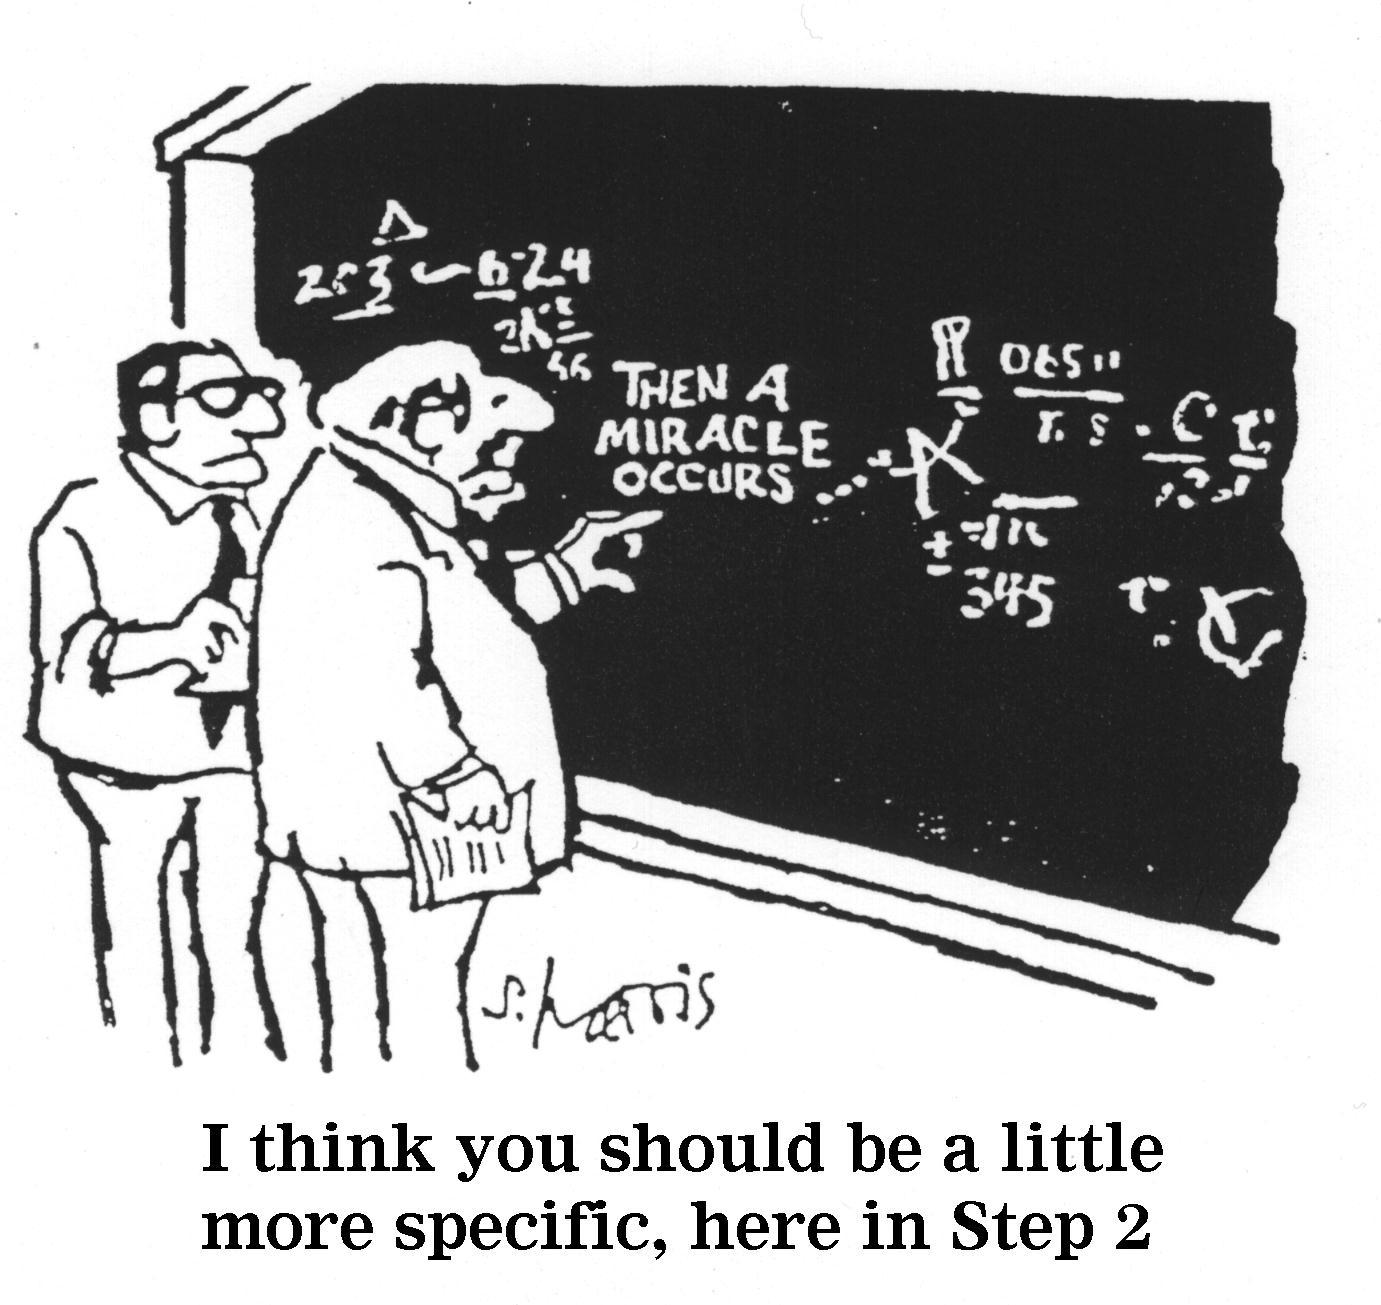
\includegraphics[width=0.4\textwidth]{images/miracle.jpeg}
\end{center}

But speculative execution inside your head is harder for perf than debugging.

So: we want to use tools \\ 
and do this in a methodical way.
\end{changemargin}

\end{frame}


%%%%%%%%%%%%%%%%%%%%%%%%%%%%%%%%%%%%%%%%%%%%%%%%%%%%%%%%%%%%%%%%%%%%%%%%%%%%%%%%
\begin{frame}
  \frametitle{Introduction to Profiling}



\begin{changemargin}{1.5cm}
    So far we've been looking at small problems.\\[1em]
    Must {\bf profile} to see what's slow in a
      large program.\\[1em]
    Two main outputs:
      \begin{itemize}
        \item flat;
        \item call-graph.
      \end{itemize}



    Two main data gathering methods:
      \begin{itemize}
        \item statistical;
        \item instrumentation.
      \end{itemize}
   \end{changemargin}
\end{frame}
%%%%%%%%%%%%%%%%%%%%%%%%%%%%%%%%%%%%%%%%%%%%%%%%%%%%%%%%%%%%%%%%%%%%%%%%%%%%%%%%

%%%%%%%%%%%%%%%%%%%%%%%%%%%%%%%%%%%%%%%%%%%%%%%%%%%%%%%%%%%%%%%%%%%%%%%%%%%%%%%%
\begin{frame}
  \frametitle{Profiler Outputs}


\begin{changemargin}{.5cm}
  
  {\bf Flat Profiler:}

  \begin{itemize}
    \item Only computes average time in a particular function.
    \item Does not include other (useful) information (callees).
  \end{itemize}

~\\[1em]

  {\bf Call-graph Profiler:}

  \begin{itemize}
    \item Computes call times.
    \item Reports frequency of function calls.
    \item Gives a call graph: who called what function?
  \end{itemize}
  \end{changemargin}
\end{frame}
%%%%%%%%%%%%%%%%%%%%%%%%%%%%%%%%%%%%%%%%%%%%%%%%%%%%%%%%%%%%%%%%%%%%%%%%%%%%%%%%

%%%%%%%%%%%%%%%%%%%%%%%%%%%%%%%%%%%%%%%%%%%%%%%%%%%%%%%%%%%%%%%%%%%%%%%%%%%%%%%%
\begin{frame}
  \frametitle{Data Gathering Methods}


\begin{changemargin}{1.5cm}
  {\bf Statistical:}

  Mostly, take samples of the system state, that is:
  \begin{itemize}
    \item every 100ms, check the system state.
    \item will cause some slowdown, but not much.
  \end{itemize}
~\\[1em]

  {\bf Instrumentation:}\\
  Add instructions at specified program points:
  \begin{itemize}
    \item can do this at compile time or run time (expensive);
    \item can instrument either manually or automatically;
    \item like conditional breakpoints.
  \end{itemize}
  \end{changemargin}
\end{frame}
%%%%%%%%%%%%%%%%%%%%%%%%%%%%%%%%%%%%%%%%%%%%%%%%%%%%%%%%%%%%%%%%%%%%%%%%%%%%%%%%

%%%%%%%%%%%%%%%%%%%%%%%%%%%%%%%%%%%%%%%%%%%%%%%%%%%%%%%%%%%%%%%%%%%%%%%%%%%%%%%%
\begin{frame}
  \frametitle{Guide to Profiling}

  

\begin{changemargin}{1cm}
  When writing large software projects:\\[1em]

     $\bullet$ First, write clear and concise code. \\
      \qquad Don't do premature optimizations---\\
      \qquad focus on correctness.\\
     $\bullet$ Profile to get a baseline of your performance:\\[0em]
      \begin{itemize}
        \item allows you to easily track any performance changes;
        \item allows you to re-design your program before it's too late.
      \end{itemize}
  Focus your optimization efforts on the code that matters.
  \end{changemargin}
\end{frame}
%%%%%%%%%%%%%%%%%%%%%%%%%%%%%%%%%%%%%%%%%%%%%%%%%%%%%%%%%%%%%%%%%%%%%%%%%%%%%%%%

%%%%%%%%%%%%%%%%%%%%%%%%%%%%%%%%%%%%%%%%%%%%%%%%%%%%%%%%%%%%%%%%%%%%%%%%%%%%%%%%
\begin{frame}
  \frametitle{Things to Look For}


\begin{changemargin}{1.5cm}
  
    Good signs:\\[0em]

    \begin{itemize}
      \item Time is spent in the right part of the system.
      \item Most time should not be spent handling errors;\\
 in non-critical code; or in exceptional cases.
      \item Time is not unnecessarily spent in OS.
    \end{itemize}
    \end{changemargin}
    
    \begin{center}
	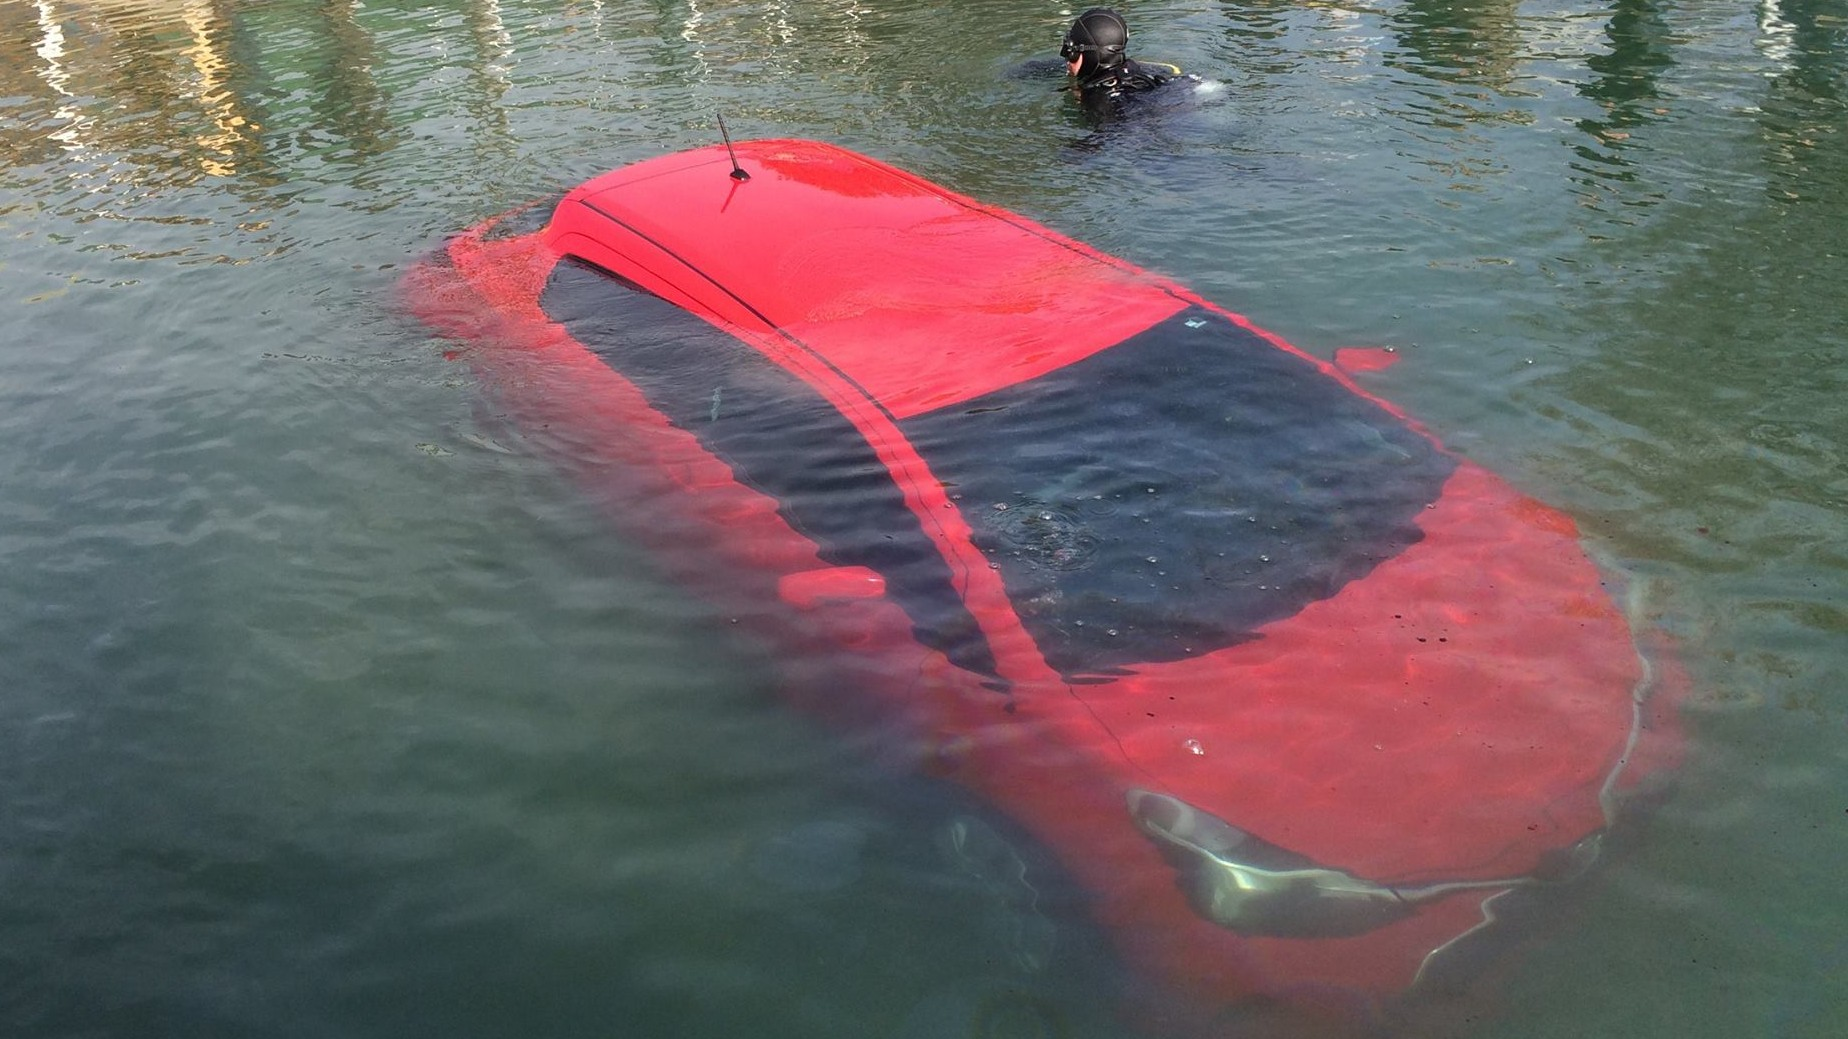
\includegraphics[width=0.5\textwidth]{images/tobermory.jpg}\\
	\hfill Kitchener driver follows GPS directions right into Lake Huron...
 	\end{center}
    
\end{frame}
%%%%%%%%%%%%%%%%%%%%%%%%%%%%%%%%%%%%%%%%%%%%%%%%%%%%%%%%%%%%%%%%%%%%%%%%%%%%%%%%


\begin{frame}
\frametitle{Development vs Prod}

You can always profile your systems in development, but that might not
help with complexities in production. 

The constraints on profiling 
production systems are that the profiling must not affect the system's
performance or reliability.


\end{frame}


\begin{frame}
\frametitle{Per-Process}

 We'll first talk about {\tt perf}, the profiler 
recommended for use with Rust. This is Linux-specific, though.

The \texttt{perf} tool is an interface to the Linux kernel's built-in
sample-based profiling using CPU counters. 

\end{frame}


\begin{frame}[fragile]
\frametitle{Previous Offering Profiling}

\begin{lstlisting}[basicstyle=\scriptsize]
[plam@lynch nm-morph]$ perf stat ./test_harness

 Performance counter stats for './test_harness':

       6562.501429 task-clock                #    0.997 CPUs utilized          
               666 context-switches          #    0.101 K/sec                  
                 0 cpu-migrations            #    0.000 K/sec                  
             3,791 page-faults               #    0.578 K/sec                  
    24,874,267,078 cycles                    #    3.790 GHz                     [83.32%]
    12,565,457,337 stalled-cycles-frontend   #   50.52% frontend cycles idle    [83.31%]
     5,874,853,028 stalled-cycles-backend    #   23.62% backend  cycles idle    [66.63%]
    33,787,408,650 instructions              #    1.36  insns per cycle        
                                             #    0.37  stalled cycles per insn [83.32%]
     5,271,501,213 branches                  #  803.276 M/sec                   [83.38%]
       155,568,356 branch-misses             #    2.95% of all branches         [83.36%]

       6.580225847 seconds time elapsed
\end{lstlisting} %$

\end{frame}

\begin{frame}[fragile]
\frametitle{Do it with Rust}

The first thing to do is to compile with debugging info, go to your \texttt{Cargo.toml} file and add:
\begin{verbatim}
[profile.release]
debug = true
\end{verbatim}

This means that \texttt{cargo build --release} will now compile the version with debug info.

\end{frame}

\begin{frame}
\frametitle{I've got a Cunning Plan}

Run the program using \texttt{perf record}, which will sample the execution of the program to produce a data set.


Then there are three ways we can look at the code: \texttt{perf report}, \texttt{perf annotate}, and a flamegraph.

\end{frame}


\begin{frame}
\frametitle{CLion}

During development of some of the code exercises, I used the CLion built-in profiler for this purpose. 

It generates a flamegraph for you too, and I'll show that for how to create the flamegraph as well.


\end{frame}



\end{document}

